\documentclass[journal]{IEEEtran}
%
% If IEEEtran.cls has not been installed into the LaTeX system files,
% manually specify the path to it like:
% \documentclass[journal]{../sty/IEEEtran}

% Some very useful LaTeX packages include:
% (uncomment the ones you want to load)


% *** MISC UTILITY PACKAGES ***
%
%\usepackage{ifpdf}
% Heiko Oberdiek's ifpdf.sty is very useful if you need conditional
% compilation based on whether the output is pdf or dvi.
% usage:
% \ifpdf
%   % pdf code
% \else
%   % dvi code
% \fi
% The latest version of ifpdf.sty can be obtained from:
% http://www.ctan.org/pkg/ifpdf
% Also, note that IEEEtran.cls V1.7 and later provides a builtin
% \ifCLASSINFOpdf conditional that works the same way.
% When switching from latex to pdflatex and vice-versa, the compiler may
% have to be run twice to clear warning/error messages.


% *** CITATION PACKAGES ***
%
%\usepackage{cite}
% cite.sty was written by Donald Arseneau
% V1.6 and later of IEEEtran pre-defines the format of the cite.sty package
% \cite{} output to follow that of the IEEE. Loading the cite package will
% result in citation numbers being automatically sorted and properly
% "compressed/ranged". e.g., [1], [9], [2], [7], [5], [6] without using
% cite.sty will become [1], [2], [5]--[7], [9] using cite.sty. cite.sty's
% \cite will automatically add leading space, if needed. Use cite.sty's
% noadjust option (cite.sty V3.8 and later) if you want to turn this off
% such as if a citation ever needs to be enclosed in parenthesis.
% cite.sty is already installed on most LaTeX systems. Be sure and use
% version 5.0 (2009-03-20) and later if using hyperref.sty.
% The latest version can be obtained at:
% http://www.ctan.org/pkg/cite
% The documentation is contained in the cite.sty file itself.

% *** GRAPHICS RELATED PACKAGES ***
%
\ifCLASSINFOpdf
\usepackage[pdftex]{graphicx}
% declare the path(s) where your graphic files are
% \graphicspath{{../pdf/}{../jpeg/}}
% and their extensions so you won't have to specify these with
% every instance of \includegraphics
% \DeclareGraphicsExtensions{.pdf,.jpeg,.png}
\else
% or other class option (dvipsone, dvipdf, if not using dvips). graphicx
% will default to the driver specified in the system graphics.cfg if no
% driver is specified.
% \usepackage[dvips]{graphicx}
% declare the path(s) where your graphic files are
% \graphicspath{{../eps/}}
% and their extensions so you won't have to specify these with
% every instance of \includegraphics
% \DeclareGraphicsExtensions{.eps}
\fi
% graphicx was written by David Carlisle and Sebastian Rahtz. It is
% required if you want graphics, photos, etc. graphicx.sty is already
% installed on most LaTeX systems. The latest version and documentation
% can be obtained at:
% http://www.ctan.org/pkg/graphicx
% Another good source of documentation is "Using Imported Graphics in
% LaTeX2e" by Keith Reckdahl which can be found at:
% http://www.ctan.org/pkg/epslatex
%
% latex, and pdflatex in dvi mode, support graphics in encapsulated
% postscript (.eps) format. pdflatex in pdf mode supports graphics
% in .pdf, .jpeg, .png and .mps (metapost) formats. Users should ensure
% that all non-photo figures use a vector format (.eps, .pdf, .mps) and
% not a bitmapped formats (.jpeg, .png). The IEEE frowns on bitmapped formats
% which can result in "jaggedy"/blurry rendering of lines and letters as
% well as large increases in file sizes.
%
% You can find documentation about the pdfTeX application at:
% http://www.tug.org/applications/pdftex

% *** MATH PACKAGES ***
%
\usepackage{amsmath}
% A popular package from the American Mathematical Society that provides
% many useful and powerful commands for dealing with mathematics.
%
% Note that the amsmath package sets \interdisplaylinepenalty to 10000
% thus preventing page breaks from occurring within multiline equations. Use:
%\interdisplaylinepenalty=2500
% after loading amsmath to restore such page breaks as IEEEtran.cls normally
% does. amsmath.sty is already installed on most LaTeX systems. The latest
% version and documentation can be obtained at:
% http://www.ctan.org/pkg/amsmath


% *** SUBFIGURE PACKAGES ***
\ifCLASSOPTIONcompsoc
\usepackage[caption=false,font=normalsize,labelfont=sf,textfont=sf]{subfig}
\else
\usepackage[caption=false,font=footnotesize]{subfig}
\fi

\usepackage{tikz}
\usetikzlibrary{shapes.geometric, arrows, calc}
\tikzstyle{startstop} = [rectangle, rounded corners, minimum width=3cm, minimum height=0.5cm,text centered, draw=black, fill=white!30, ]
\tikzstyle{process} = [rectangle, minimum width=3cm, minimum height=0.5cm, text centered, draw=black, fill=white!30]
\tikzstyle{decision} = [diamond, minimum width=3cm, minimum height=1cm, text centered, draw=black, fill=green!30]
\tikzstyle{arrow} = [thick,->,>=stealth]

\usepackage{hyperref}

\begin{document}
%
% paper title
% Titles are generally capitalized except for words such as a, an, and, as,
% at, but, by, for, in, nor, of, on, or, the, to and up, which are usually
% not capitalized unless they are the first or last word of the title.
% Linebreaks \\ can be used within to get better formatting as desired.
% Do not put math or special symbols in the title.
    \title{Preliminary Report for a Motion Detection System}
%
%
% author names and IEEE memberships
% note positions of commas and nonbreaking spaces ( ~ ) LaTeX will not break
% a structure at a ~ so this keeps an author's name from being broken across
% two lines.
% use \thanks{} to gain access to the first footnote area
% a separate \thanks must be used for each paragraph as LaTeX2e's \thanks
% was not built to handle multiple paragraphs
%

    \author{Joey Hines}

% The paper headers
    \markboth{ELEC 7340: Digital Image Processing Preliminary Report}%
    {Shell \MakeLowercase{\textit{et al.}}: ELEC 7340: Digital Image Processing Preliminary Report}


% make the title area
    \maketitle

% As a general rule, do not put math, special symbols or citations
% in the abstract or keywords.
    \begin{abstract}
        As camera sensors and processors have become cheaper, a wave of cheap, self-contained video surveillance solutions have entered
        the market. A popular application of these cameras is using them for motion detection. While many motion detection algorithm have
        been presented, this project aims to create one that is easily implementable on a low-end hardware target such as a Raspberry Pi
    \end{abstract}


% For peer review papers, you can put extra information on the cover
% page as needed:
% \ifCLASSOPTIONpeerreview
% \begin{center} \bfseries EDICS Category: 3-BBND \end{center}
% \fi
%
% For peerreview papers, this IEEEtran command inserts a page break and
% creates the second title. It will be ignored for other modes.
    \IEEEpeerreviewmaketitle


    \section{Introduction}
% The very first letter is a 2 line initial drop letter followed
% by the rest of the first word in caps.
%
% form to use if the first word consists of a single letter:
% \IEEEPARstart{A}{demo} file is ....
%
% form to use if you need the single drop letter followed by
% normal text (unknown if ever used by the IEEE):
% \IEEEPARstart{A}{}demo file is ....
%
% Some journals put the first two words in caps:
% \IEEEPARstart{T}{his demo} file is ....
%
% Here we have the typical use of a "T" for an initial drop letter
% and "HIS" in caps to complete the first word.
    \IEEEPARstart{V}{ideo} surveillance has become more affordable in the last several years as costs of camera sensors and processors have dropped. With more video cameras than ever, it is important to be able to sift through video of nothing to find
    frames on interests. Commonly, this is done with motion detection. Frames of video are analyzed to determine if motion has
    occurred in the video.

    This detection algorithm needs to be sensitive to motion and ideally not be set off by false alarms such as changes in light or
    dynamic objects within the scene. Consumers also expect camera units to be all-in-one. Meaning each camera
    should handle storing video and analyzing it for motion. As these cameras also need to be inexpensive, that often means cheaper
    and less advanced processors are used. The challenge then becomes marking a motion detection algorithm that is lightweight
    enough to run on a cheaper processor and good enough to not set off false alarms. This project aims to implement such a
    system, targeting a Raspberry Pi. This report first dives into related work in motion detection. Then, an efficient algorithm
    is proposed. Last, current work completed is discussed.

    \section{Related Works}
    One early example \cite{Jain} of this process uses differences between images to detect events occurring in the video. It uses a
    process known as first-order difference picture (FODP). A FODP is built by comparing a sequence of frames. Each time a region
    of a frame has a difference detected, the corresponding FODP pixel is incremented by one. Effectively each pixel is a count of
    how different the pixels is from the original frame. This paper also presents the idea of using a single frame as a background
    model.

    In more recent years, further advances have been built upon similar concepts such as\cite{Sing}.
    This paper presents a lot of common issues that any motion detection algorithm may face. This includes illumination changes,
    dynamic objects in background, shadows, bootstrapping and video noise. Each of these will be further discussed later. The
    algorithm proposed constructs a background model from an initial model. Further frames are then analyzed for motion detection.
    It also presents methods to mitigate the effects of background objects being removed from the frame, refereed to as ghosts. It
    employs a \emph{l-g-r} color method which aims to separate luminosity from color information.

    Another recent paper \cite{Gaba} presents a method for using multiple frames to establish the background image. This helps
    prevent objects moving during bootstrapping from ghosting on the image. To generate the background model, a moving average is
    used to generate the background model. This model is then  subtracted from the current image to detect motion within the image.
    This paper also presents how the track the predicted path of objects. This allows for objects to be easily tracked in the scene
    and to prevent ghosting on the model.

    \cite{Sehairi_2017} is a report that compares many methods of motion detection and explains the algorithms. The algorithm presented that
    preforms the best is knows as Eigen-background Subtraction from \cite{Oliver}. The paper itself is applying motion detection to tracking
    human interactions, but its method for motion  detection seems very versatile. It builds a background model by making an eigenspace model.
    This model is created by finding the mean image of several sequential images and finding a covariance matrix. The eigenspace matrix is then
    built by using eigenvalue decommission. The largest of these eigenvalues are kept. Input images are then projected the space defined by
    the eigenvalues to build the model. To detect motion, the input image is subtracted from the background model to detect motion in the
    image.

    \section{Proposed Algorithm}
    \cite{Gaba}, \cite{Jain}, \cite{Oliver}, and to some some extent \cite{Jain}, follow the same basic algorithm.
    They begin the process of first modeling the background of image. This allows the system to know
    when any changes have occurred. What sets apart these systems is how they model the background and how they
    handle object tracking in the scene. As discussed in \cite{Sing}, several common issues come up in motion detection. One of the
    biggest is changes in luminosity. As lights turn on or clouds block the sun, light in a scene will be constantly changing.
    Ideally, light changes should not be detected as motion. Dynamic items in a scene can also impact the capability of the system.
    Fans or other constant movement should not cause false alarms in detection. \cite{Oliver} algorithm seems to minimize a lot of these
    issues, but required a large amount of matrix operations.

    \subsection{Color System}
    Without reinventing the wheel for color systems, the HSL (Hue, Saturation, Lightness) color system will be used to conduct
    analysis on images. This is similar to the color system discussed in \cite{Gaba}, where colors are broken up into the color
    components and their luminosity. By looking at just changes in the Hue and Saturation channels, luminosity can be ignored.

    \subsection{Background Model}
    The background model of the image will be generated by a moving average of the current frame. The modification of the
    moving average will be similar to the one proposed in \cite{Gaba}. The background model, $\mathbf{B_n}$ is initially given by:
    $$
    \mathbf{B}_n = \mathbf{B}_{n-1} + \frac{1}{N}\mathbf{F}_n
    $$
    Where $N$ is the number of frames to keep in the model ($N=10$) and $\mathbf{}{F_n}$ is the current frame being captured by the image. After N frames, the model will be generated by the following:
    $$
    \mathbf{B}_n = \mathbf{B}_{n-1} + \frac{1}{N}(\mathbf{F}_n - \mathbf{F}_{n-N})
    $$
    Where $ \mathbf{F}_{n-N}$ is the oldest frame in the model. This keeps the model updated only on current data and helps eliminate
    ghosting issues as discussed in \cite{Sing}.

    \subsection{Motion Mask}
    The Motion Mask is similar to a FODP found in \cite{Jain}. The Motion Mask is an array of \texttt{double} values the same size as the original image. Each value is initialized to a $1.0$. The difference from FODP is that instead of incriminating a pixel when
    the image is different than a base frame, a value in the Motion Mask is decremented slightly when a motion is detected in the
    corresponding pixel on the source frame. If a pixel in the source image is often setting off the detector, it likely means
    it is a dynamic part of the background  and the system should becomes less sensitive to this. A value within the Motion Mask
    is incremented if a pixel does not contain motion. This allows the system to recover from changes in the background.

    \begin{figure}[!t]
        \centering
        \caption{Proposed Algorithm}
        \label{fig:algorithm}
        \begin{tikzpicture}[node distance=1cm]
            \node (start) [startstop] {Video Sequence};
            \node (bg_model) [process, below of=start] {Build Background Model};
            \node (bg_sub) [process, below of=bg_model] {Subtract Out Background};
            \node (motion_mask) [process, below of=bg_sub] {Apply Motion Mask};
            \node (threshold) [process, below of=motion_mask] {Threshold};
            \node (filter) [process, below of=threshold] {Apply Low-Pass Filter};
            \node (edge_detect) [process, below of=filter] {Edge Detect};
            \node (draw_box) [process, below of=edge_detect] {Draw Motion Box};
            \node (update_bg_model) [process, below of=draw_box] {Update BG Model/Motion Mask};
            \node (display) [process, below of= update_bg_model] {Display output};
            \coordinate (flow) at ($(display.east)+(1.2cm,0)$);

            \draw [arrow] (start) -- (bg_model);
            \draw [arrow] (bg_model) -- (bg_sub);
            \draw [arrow] (bg_sub) -- (motion_mask);
            \draw [arrow] (motion_mask) -- (threshold);
            \draw [arrow] (threshold) -- (filter);
            \draw [arrow] (filter) -- (edge_detect);
            \draw [arrow] (edge_detect) -- (draw_box);
            \draw [arrow] (draw_box) -- (update_bg_model);
            \draw [arrow] (update_bg_model) -- (display);
            \draw [arrow] (display) -- (flow) |-  (bg_sub);
        \end{tikzpicture}
    \end{figure}

    \subsection{Detecting Motion}
    The algorithm for the process of detecting motion is shown in Figure \ref{fig:algorithm}. First a difference is found between the
    current frame and the background model:
    $$
    \mathbf{D}_n = \lfloor\mathbf{B}_n - \mathbf{I}_n\rfloor
    $$
    Where $\mathbf{B}_n$ is the current background model, $\mathbf{I_n}$ is the current frame. This removes background elements from the image leaving only moving objects.The output of the difference process is then point-wise multiplied by the motion mask:
    $$
    \mathbf{F}_n = \mathbf{D}_n \circ \mathbf{M}_n
    $$
    Where $\mathbf{M}_n$ is the motion mask.This darkens areas of the image where motion commonly occurs. The scaled image is thresholded such
    that regions that contain motion are white and ignored regions are black.
    This threshold  image is then passed through a smoothing filter to remove smaller regions. Sobel operators are used on the smooth threshold
    image to find edges of the motion. Both the Sobel operation and filtering can be implemented by convolution. The min and max values of the edges are found to find a bounding box around the motion that can then be displayed on the original image.

    \section{Work Completed}
    So far, most progress has been made in gathering the image from a video source on Linux. Current;y, a program has
    been written that opens a video source on a Linux computer and displays the output the frame and a simple background model. Code
    written for the project so far can be found in Appendix A.

    \subsection{Capturing Video}
    To handle opening a video source and getting frames from it, Video For Linux (V4L) is used. V4L is a fairly low level API but
    supports virtually all video sources that Linux has drivers for. it also very lightweight which is perfect for the target
    RaspberryPI. Being a low level API, it also very complicated with a lot of setup and dense documentation. A lot of time was needed to get the camera  properly opened and outputting video. The webcam on the development computer outputs compressed MJPEG
    and YVYU images. YVYU will likely be used at its not compressed.

    \subsection{Displaying Video}
    Simple Direct Media-Layer (SDL) is used to display the raw frames acquired from the webcam. SDL handles a lot of the GUI aspects
    such as opening a Window and displaying the image. It also has good threading support allowing the display and capture logic
    to run in separate threads. It also is cross-platform, and can run on the target Raspberry Pi. One of the reasons SDL was chosen
    over a simpler GUI API is its support for OpenGL. The goal being to use possibly use the GPU of the Raspberry Pi to help
    accelerate processing. SDL also allows supports things like drawing graphics on screen, which is good for handling the motion
    boxes.

    \subsection{Difference Output}
    As a test, the program currently differences the current frame with the last frame. This provides a basic form of motion
    detection. When the scene is still, a solid background is displayed as seen in Figure \ref{fig:diff_output}.a. The image is
    almost completely green except for a thin line of motion from a shirt. \ref{fig:diff_output}.b shows what happens when motion
    occurs in the frame. Everywhere that is a lighter green has had a change occurred from the previous frame This shows the moving
    portions of the image. This process will form the basis for implementing the rest of the image processing algorithm.

    \begin{figure}[!t]
        \centering
        \caption{Proposed Algorithm}
        \label{fig:diff_output}
        \subfloat[Motionless Output]{
            
\includegraphics[width=1.5in]{still.png}
        }
        \subfloat[Motion Output]{
            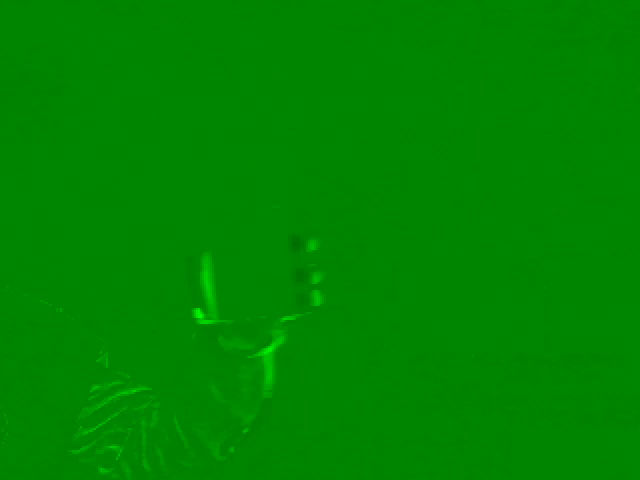
\includegraphics[width=1.5in]{motion.png}
        }
    \end{figure}

    \section{Next Steps}
    The next step of this project is to begin implementing the proposed algorithm in code and begin testing. Tweaks are expected to
    be needed in order to get the system properly detecting motion. It is important to make sure the algorithm preforms well before
    attempting to port it to the Raspberry Pi target. Performance will have to be considered as the project progress. As
    mentioned earlier, SDL supports using a GPU for acceleration. This may be invoked to increase the frame rate of the motion
    detection algorithm. If the algorithm can not process frames fast enough, there will be larger gaps between frames which may
    lead to more false positives.

    \section{Conclusion}
    While many motion detection currently exist, many are complex and require a lot of floating point operations to properly
    implement. This becomes a problem while targeting simple home surveillance cameras with limited processing power. The algorithm
    in this paper aims to be simpler and more efficient than most existing algorithms while minimizing false positives.

    \appendices
    \section{Code}
    The code written for this project can be found on the project's
    \href{https://github.com/joeyahines/motion_detector}{Github Repo}. Code is written in C using \href{https://www.libsdl.org/}{SDL} for GUI rendering and \href{https://www.linuxtv.org/downloads/v4l-dvb-apis-new/uapi/v4l/v4l2.html}{V4L}. Code for capturing
    video was adapted from the \href{https://www.linuxtv.org/downloads/v4l-dvb-apis-new/uapi/v4l/capture.c.html}{Video Capture Example} in the V4L documentation.


% Can use something like this to put references on a page
% by themselves when using endfloat and the captionsoff option.
    \ifCLASSOPTIONcaptionsoff
    \newpage
    \fi



% trigger a \newpage just before the given reference
% number - used to balance the columns on the last page
% adjust value as needed - may need to be readjusted if
% the document is modified later
%\IEEEtriggeratref{8}
% The "triggered" command can be changed if desired:
%\IEEEtriggercmd{\enlargethispage{-5in}}

% references section

% can use a bibliography generated by BibTeX as a .bbl file
% BibTeX documentation can be easily obtained at:
% http://mirror.ctan.org/biblio/bibtex/contrib/doc/
% The IEEEtran BibTeX style support page is at:
% http://www.michaelshell.org/tex/ieeetran/bibtex/
    \bibliographystyle{IEEEtran}
    \bibliography{IEEEabrv,ref}

\end{document}